\documentclass[english,11pt]{beamer}

\DeclareMathOperator{\Cov}{Cov}
\DeclareMathOperator{\Var}{Var}
\DeclareMathOperator{\E}{\mathbb{E}}
\DeclareMathOperator{\Proba}{\mathbb{P}}

\newcommand{\Covb}[2]{\ensuremath{\Cov\!\left[#1,#2\right]}}
\newcommand{\Eb}[1]{\ensuremath{\E\!\left[#1\right]}}
\newcommand{\Pb}[1]{\ensuremath{\Proba\!\left[#1\right]}}
\newcommand{\Varb}[1]{\ensuremath{\Var\!\left[#1\right]}}

% norm
\newcommand{\norm}[1]{\| #1 \|}

\newcommand{\indep}{\rotatebox[origin=c]{90}{$\models$}}





\usepackage{mathptmx,amsmath,amssymb,graphicx,bibentry,bbm,babel,ragged2e}

\makeatletter

\newcommand{\noun}[1]{\textsc{#1}}
\newcommand{\jitem}[1]{\item \begin{justify} #1 \end{justify} \vfill{}}
\newcommand{\sframe}[2]{\frame{\frametitle{#1} #2}}

\newenvironment{centercolumns}{\begin{columns}[c]}{\end{columns}}
%\newenvironment{jitem}{\begin{justify}\begin{itemize}}{\end{itemize}\end{justify}}

\usetheme{Warsaw}
\setbeamertemplate{footline}[text line]{}
\setbeamercolor{structure}{fg=purple!50!blue, bg=purple!50!blue}

\setbeamersize{text margin left=15pt,text margin right=15pt}

\setbeamercovered{transparent}


\@ifundefined{showcaptionsetup}{}{%
 \PassOptionsToPackage{caption=false}{subfig}}
\usepackage{subfig}

\usepackage[utf8]{inputenc}
\usepackage[T1]{fontenc}

\usepackage{multirow}


\makeatother

\begin{document}





\title{Multiscalar models for systems of cities}

\author{J.~Raimbault$^{1,2,3,4,\ast}$\\
\texttt{$\ast$ juste.raimbault@ign.fr}
}


\institute{$^{1}$ LASTIG, IGN-ENSG\\
$^{2}$CASA, UCL\\
$^{3}$UPS CNRS 3611 ISC-PIF\\
$^{4}$UMR CNRS 8504 G{\'e}ographie-cit{\'e}s
}


\date{ECTQG 2023\\\smallskip
Session Theoretical Geography 1\\\smallskip
September 15th 2023
}

\frame{\maketitle}



\sframe{An evolutionary theory for urban systems}{

% Simulation models for the dynamics of systems of cities have been developed to capture salient stylised facts of such systems and understand underlying processes (Pumain & Reuillon, 2017). These agent-based models simulate the interactions between cities at the macroscopic scale, focusing on different dimensions such as innovation or economic exchanges. They correspond to the highest level of the multiscalar ontology described by Pumain (2011) for urban systems.



\begin{center}
	\begin{columns}
	\begin{column}{0.49\linewidth}
	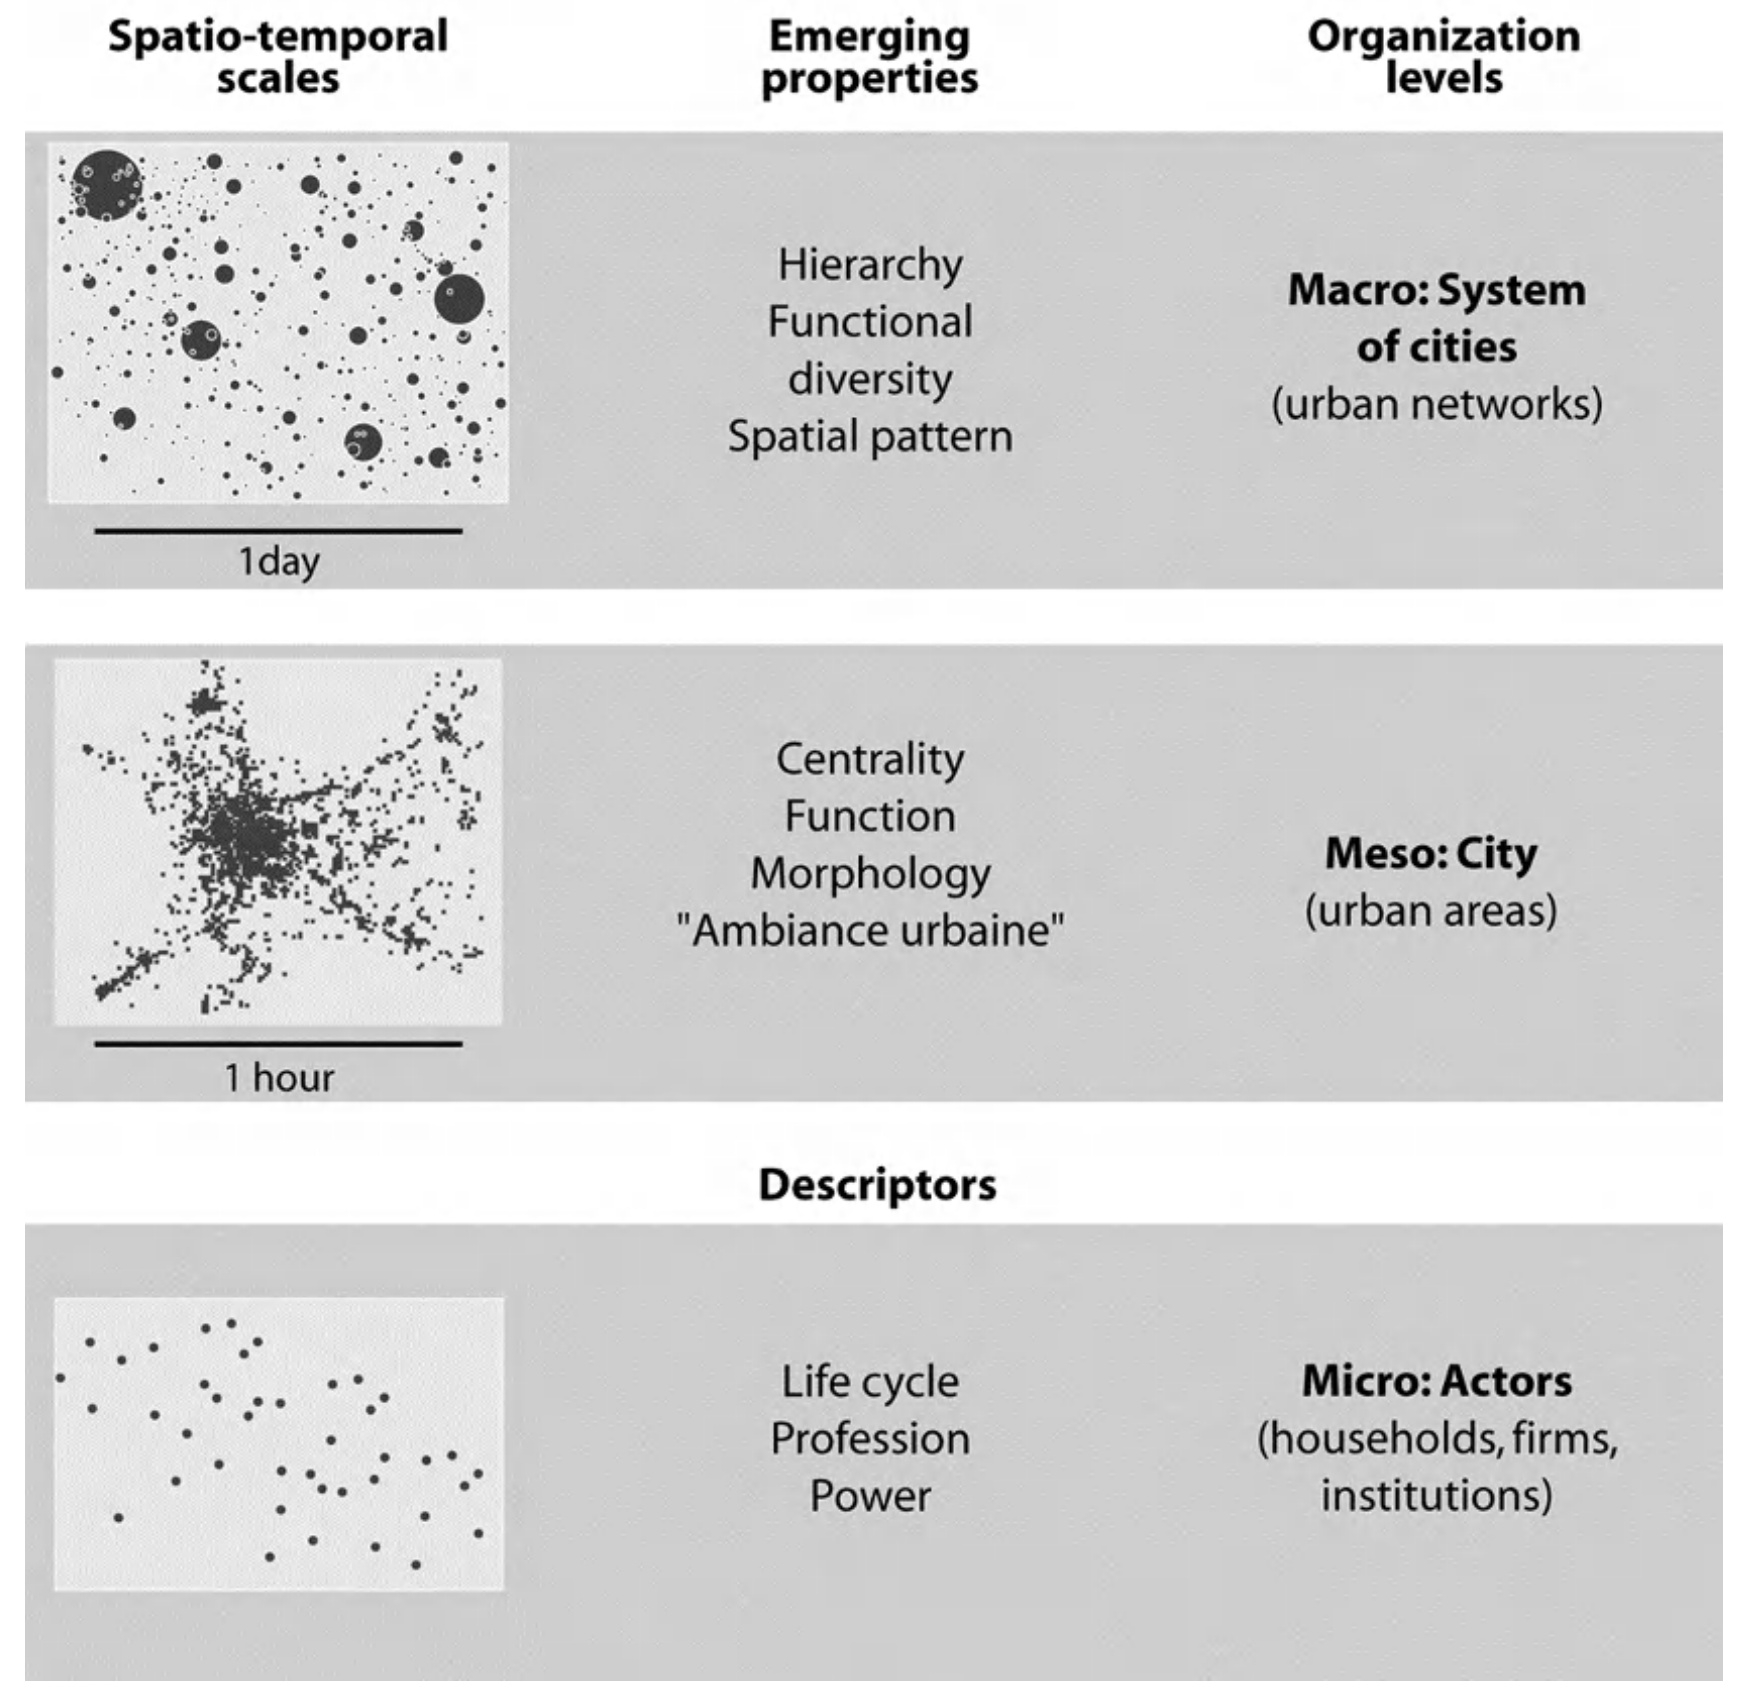
\includegraphics[width=\textwidth]{../../2020/ALife2020/figures/evoltheory_scales.png}
	\end{column}
	\begin{column}{0.3\linewidth}
	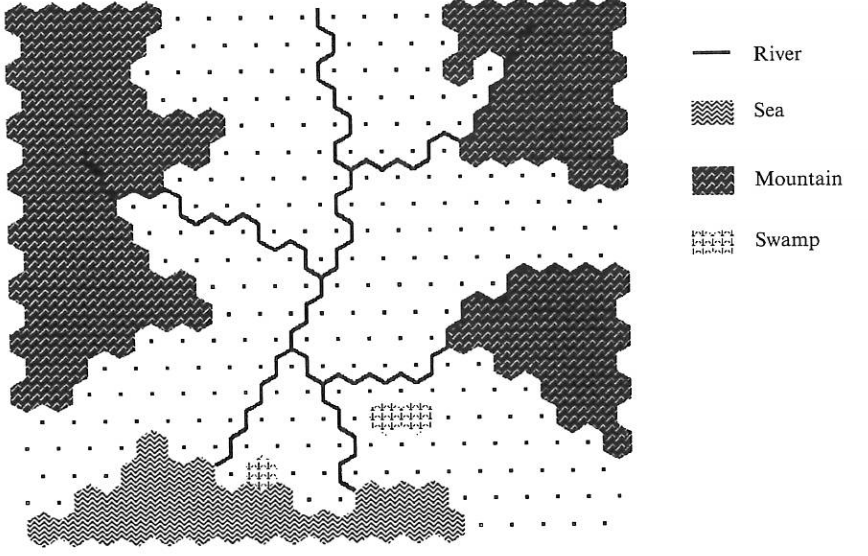
\includegraphics[width=\textwidth]{../../2020/ALife2020/figures/simpop1.png}\\\medskip
	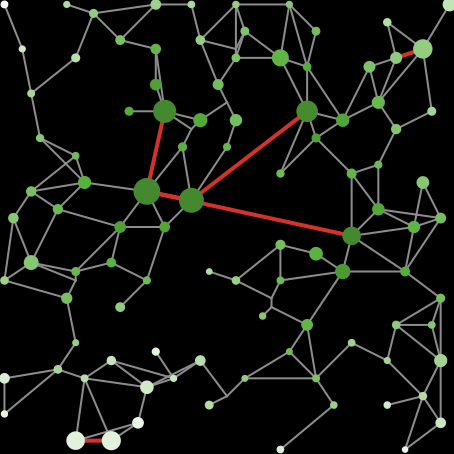
\includegraphics[width=\textwidth]{../../2020/ALife2020/figures/setup_synth_1_tick100.png}
	\end{column}
	\end{columns}
\end{center}

%\footnotesize
An evolutionary urban theory considering cities as systems within systems of cities \cite{pumain2018evolutionary}; Simpop 1 model \cite{sanders1997simpop}; SimpopNet model \cite{schmitt2014modelisation}



}


\sframe{Multi-modeling urban systems dynamics for sustainability}{

% sdg tradeoffs, multiobj ersa2022


\begin{center}
	\includegraphics[width=0.51\textwidth]{../../../Papers/SDGTradeoffs/SDGTradeoffs-paper/figures/Fig3.png}
	\includegraphics[width=0.42\textwidth]{../../../../../SDGTradeoffs/Docs/Communications/2022/FRCCS2022/figures/radar_sdgs.png}
\end{center}

Trade-offs between sustainable development goals in systems of cities \cite{raimbault2020empowering}; multi-modeling for many-objectives SDGs optimisation \cite{raimbault2022trade}

}



\sframe{Hybrid models mixing scales}{

% Lutecia and physical network: "semi-multiscale"

\begin{center}
	\includegraphics[width=0.49\textwidth]{../../../../../CityNetwork/Docs/ThesisMemoire/Final/Figures/Final/7-3-3-fig-lutecia-governance.jpg}
	\includegraphics[width=0.49\textwidth]{../../../../../NetworksTerritories/CoevolutionNwTerritories/Docs/Papers/HierarchyCoevolution/chapter/figuresraw/ex_realphysical_1975_tf.png}
\end{center}

Simulation models for systems of cities and transportation networks making a slight bridge between scales: transportation governance modeling \cite{raimbault2021introducing}; physical network self-reinforcment \cite{raimbault2020hierarchy}

}


\sframe{Towards multiscale models}{

% In order to address open issues related to multi-level governance of territorial sustainable transitions, models simulating simultaneously multiple scales are however needed (Rozenblat & Pumain, 2018).

% contribution

$\rightarrow$ multi-scale simulation models are needed to explore sustainable policies \cite{rozenblat2018conclusion}

\bigskip


$\rightarrow$ multi-scale urban models remain however underexplored in the literature

\bigskip
\bigskip

\textbf{This contribution: } \textit{to synthesise lessons from two different recent tentatives to build multi-scale urban models with a strong coupling between scales: an urban morphogenesis model \cite{raimbault2021strong} and an innovation diffusion model \cite{raimbault2023innovation}, learnt from the systematic exploration of these models using OpenMOLE \cite{reuillon2013openmole}}


}

\sframe{Urban morphology and inter-city interactions}{

% This contribution synthesises recent lessons learnt from the construction and exploration of such strongly coupled multi-scalar models. The first model couples a macroscopic population dynamics model with local urban morphogenesis models within each city (Raimbault, 2021),

% broad description of morph-intgib model: cit ccs19 and preprint

\begin{center}
\includegraphics[width=\textwidth]{../../../../../UrbanGrowth/Docs/Papers/Multiscale/paper/figures/Fig1.jpg}
\end{center}

A strong coupling explored by \cite{raimbault2021strong} between urban morphogenesis agregation-diffusion processes at the meso scale \cite{raimbault2018calibration} and interactions between cities at the macro scale \cite{raimbault2020indirect}


}

\sframe{Model exploration}{

% salient results for urbmorph-intgib

\begin{center}
\includegraphics[width=0.58\textwidth]{../../../../../UrbanGrowth/Docs/Papers/Multiscale/paper/figures/Fig5.jpg}
\includegraphics[width=0.4\textwidth]{../../../../../UrbanGrowth/Docs/Papers/Multiscale/paper/figures/Fig7.jpg}
\end{center}

\bigskip

(Left) Non-monotonous effect of policy parameters linking scales; (Right) Bi-objective optimisation of contradictory objectives across scales

}



\sframe{Multi-scale innovation dynamics}{

% while the second one simulates the diffusion of innovation between urban areas and its impact on urban growth at the macroscopic scale, and innovation cluster dynamics within each area (Raimbault & Pumain, 2023).

\begin{center}
	\includegraphics[width=0.75\textwidth]{../../../Papers/InnovationMultiscale/InnovationMultiscale-paper/slides/figures/model_4.png}
\end{center}


A bi-scale model explored by \cite{raimbault2023innovation}, coupling urban evolution based on innovation diffusion at the macro scale \cite{raimbault2020model}, with intra-urban innovation cluster dynamics between firms for the emergence of new innovations \cite{raimbault2022innovation}; quantification of strong emergence using indicators by \cite{rosas2020reconciling}


}


\sframe{Model exploration}{

\begin{center}
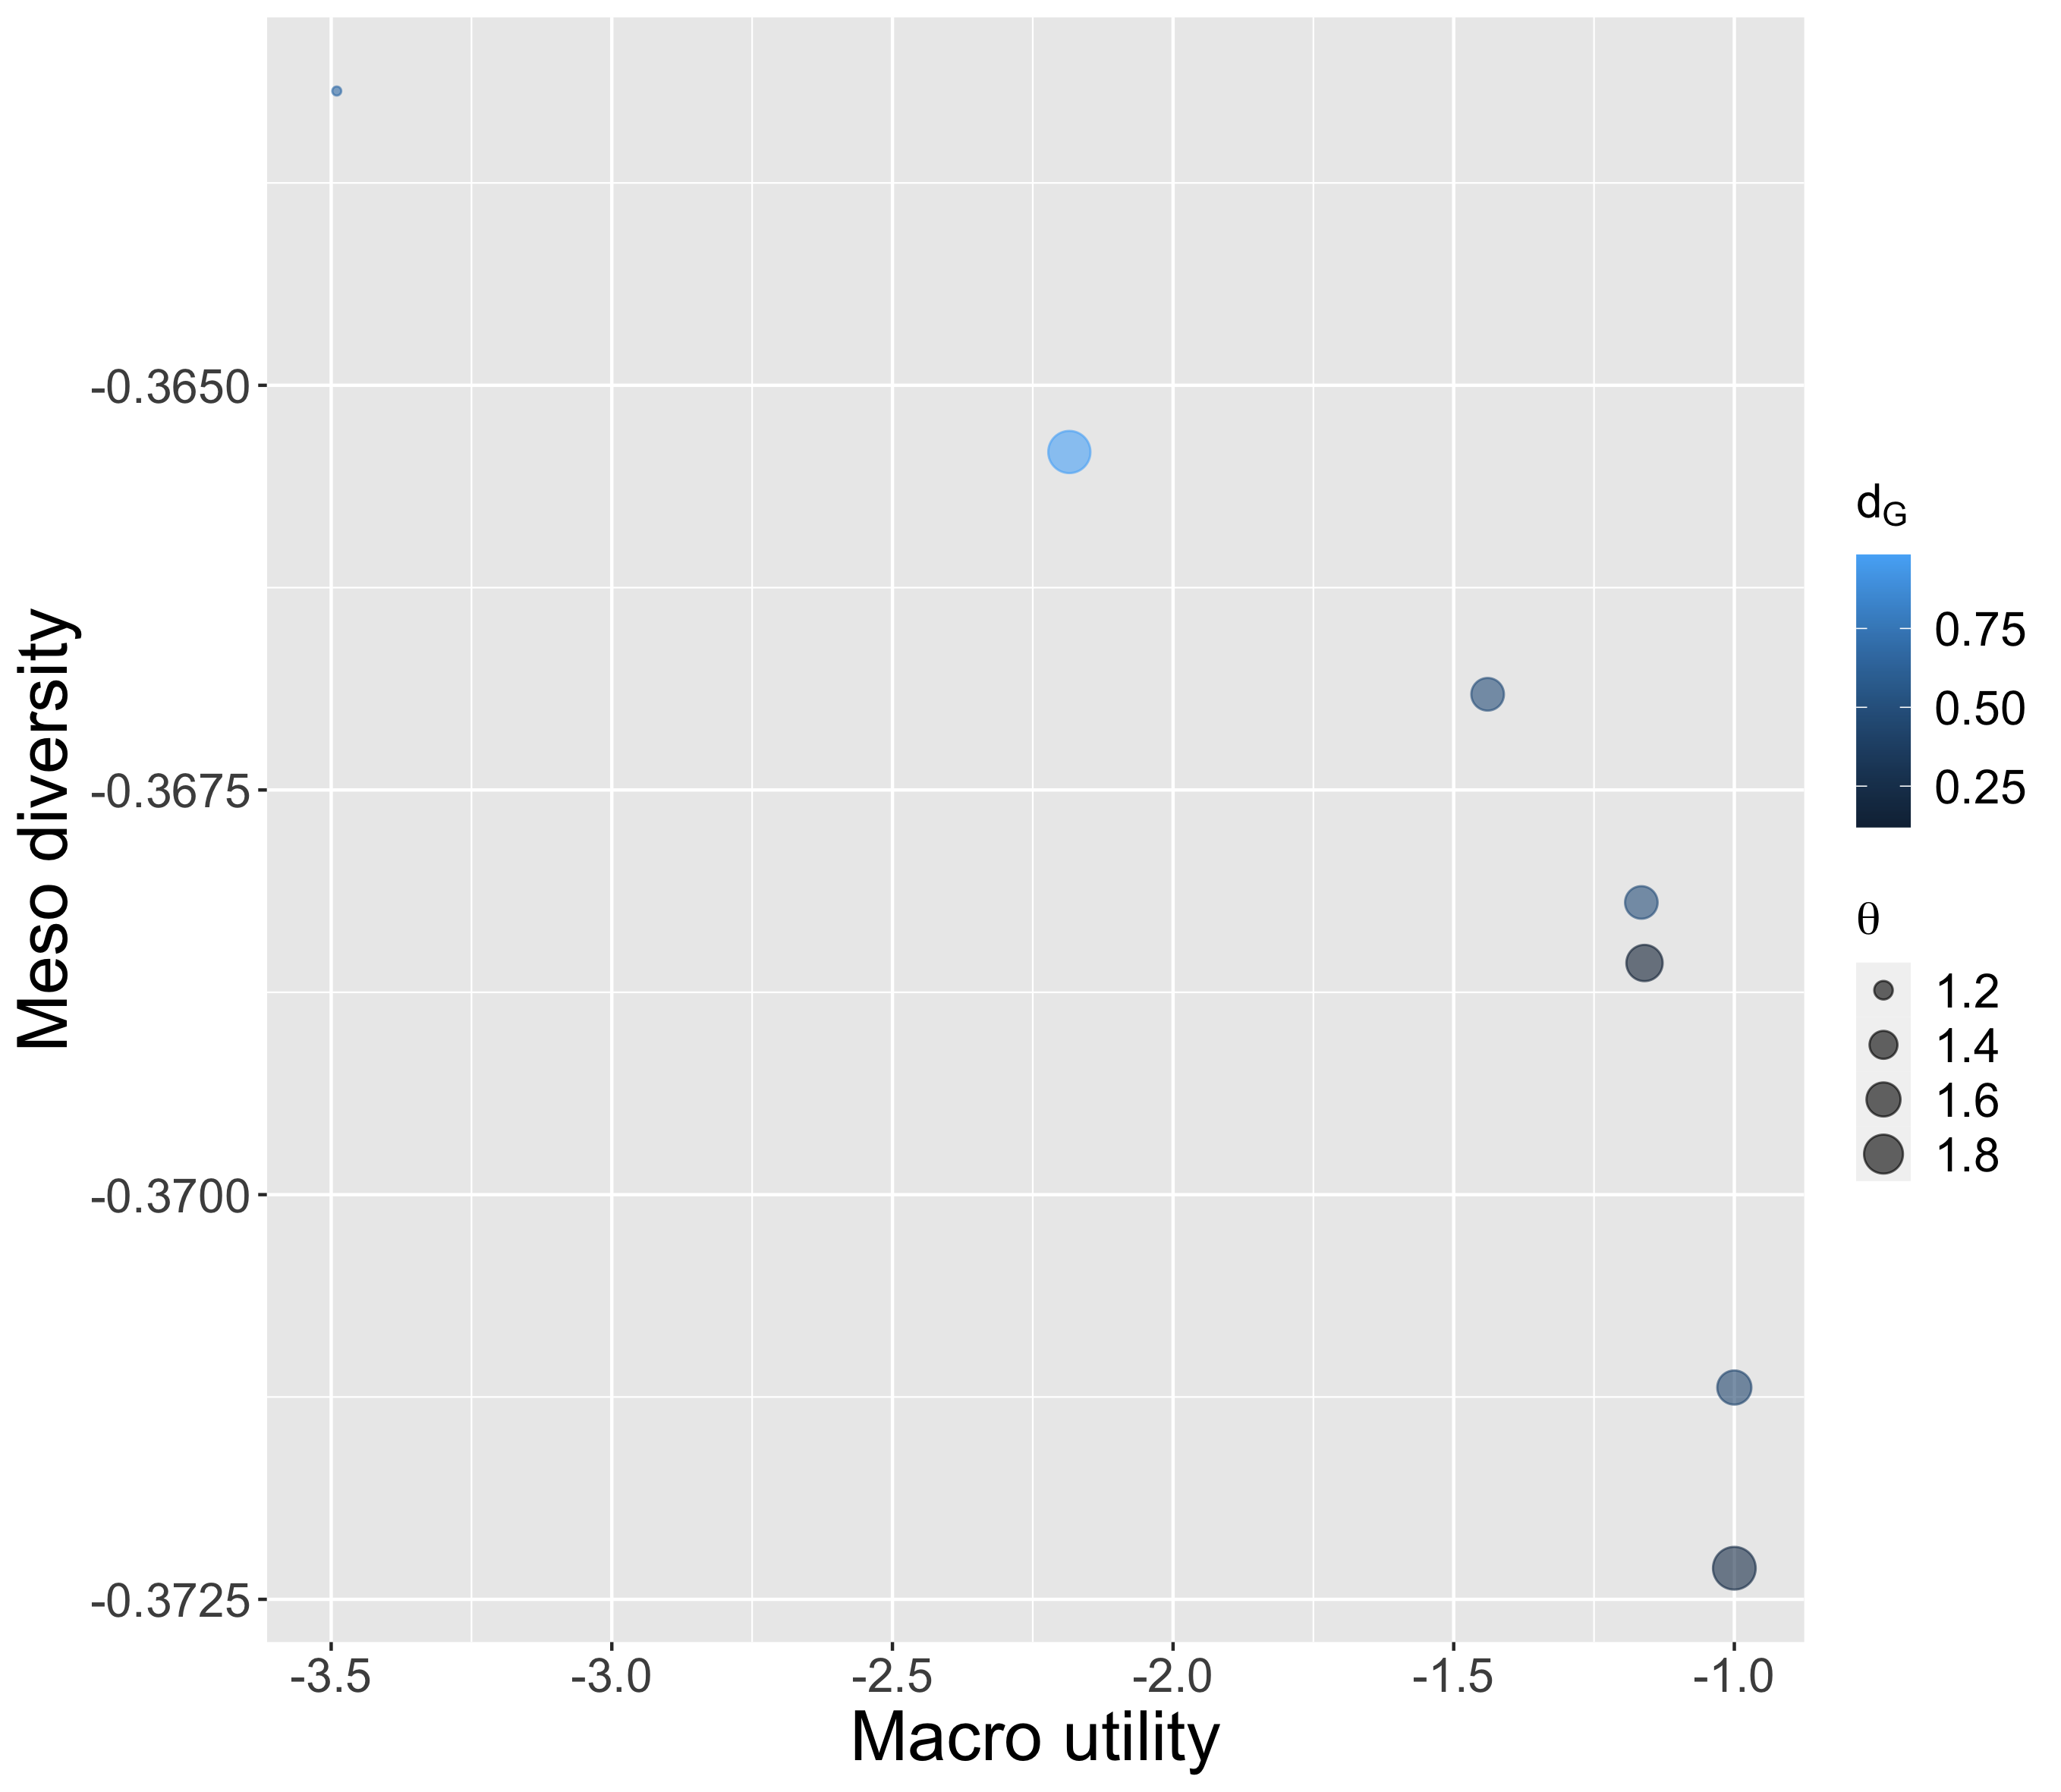
\includegraphics[width=0.49\textwidth]{../../../Papers/InnovationMultiscale/InnovationMultiscale-paper/figures/paretoDiversity-Fitness_colordG_sizetheta.png}
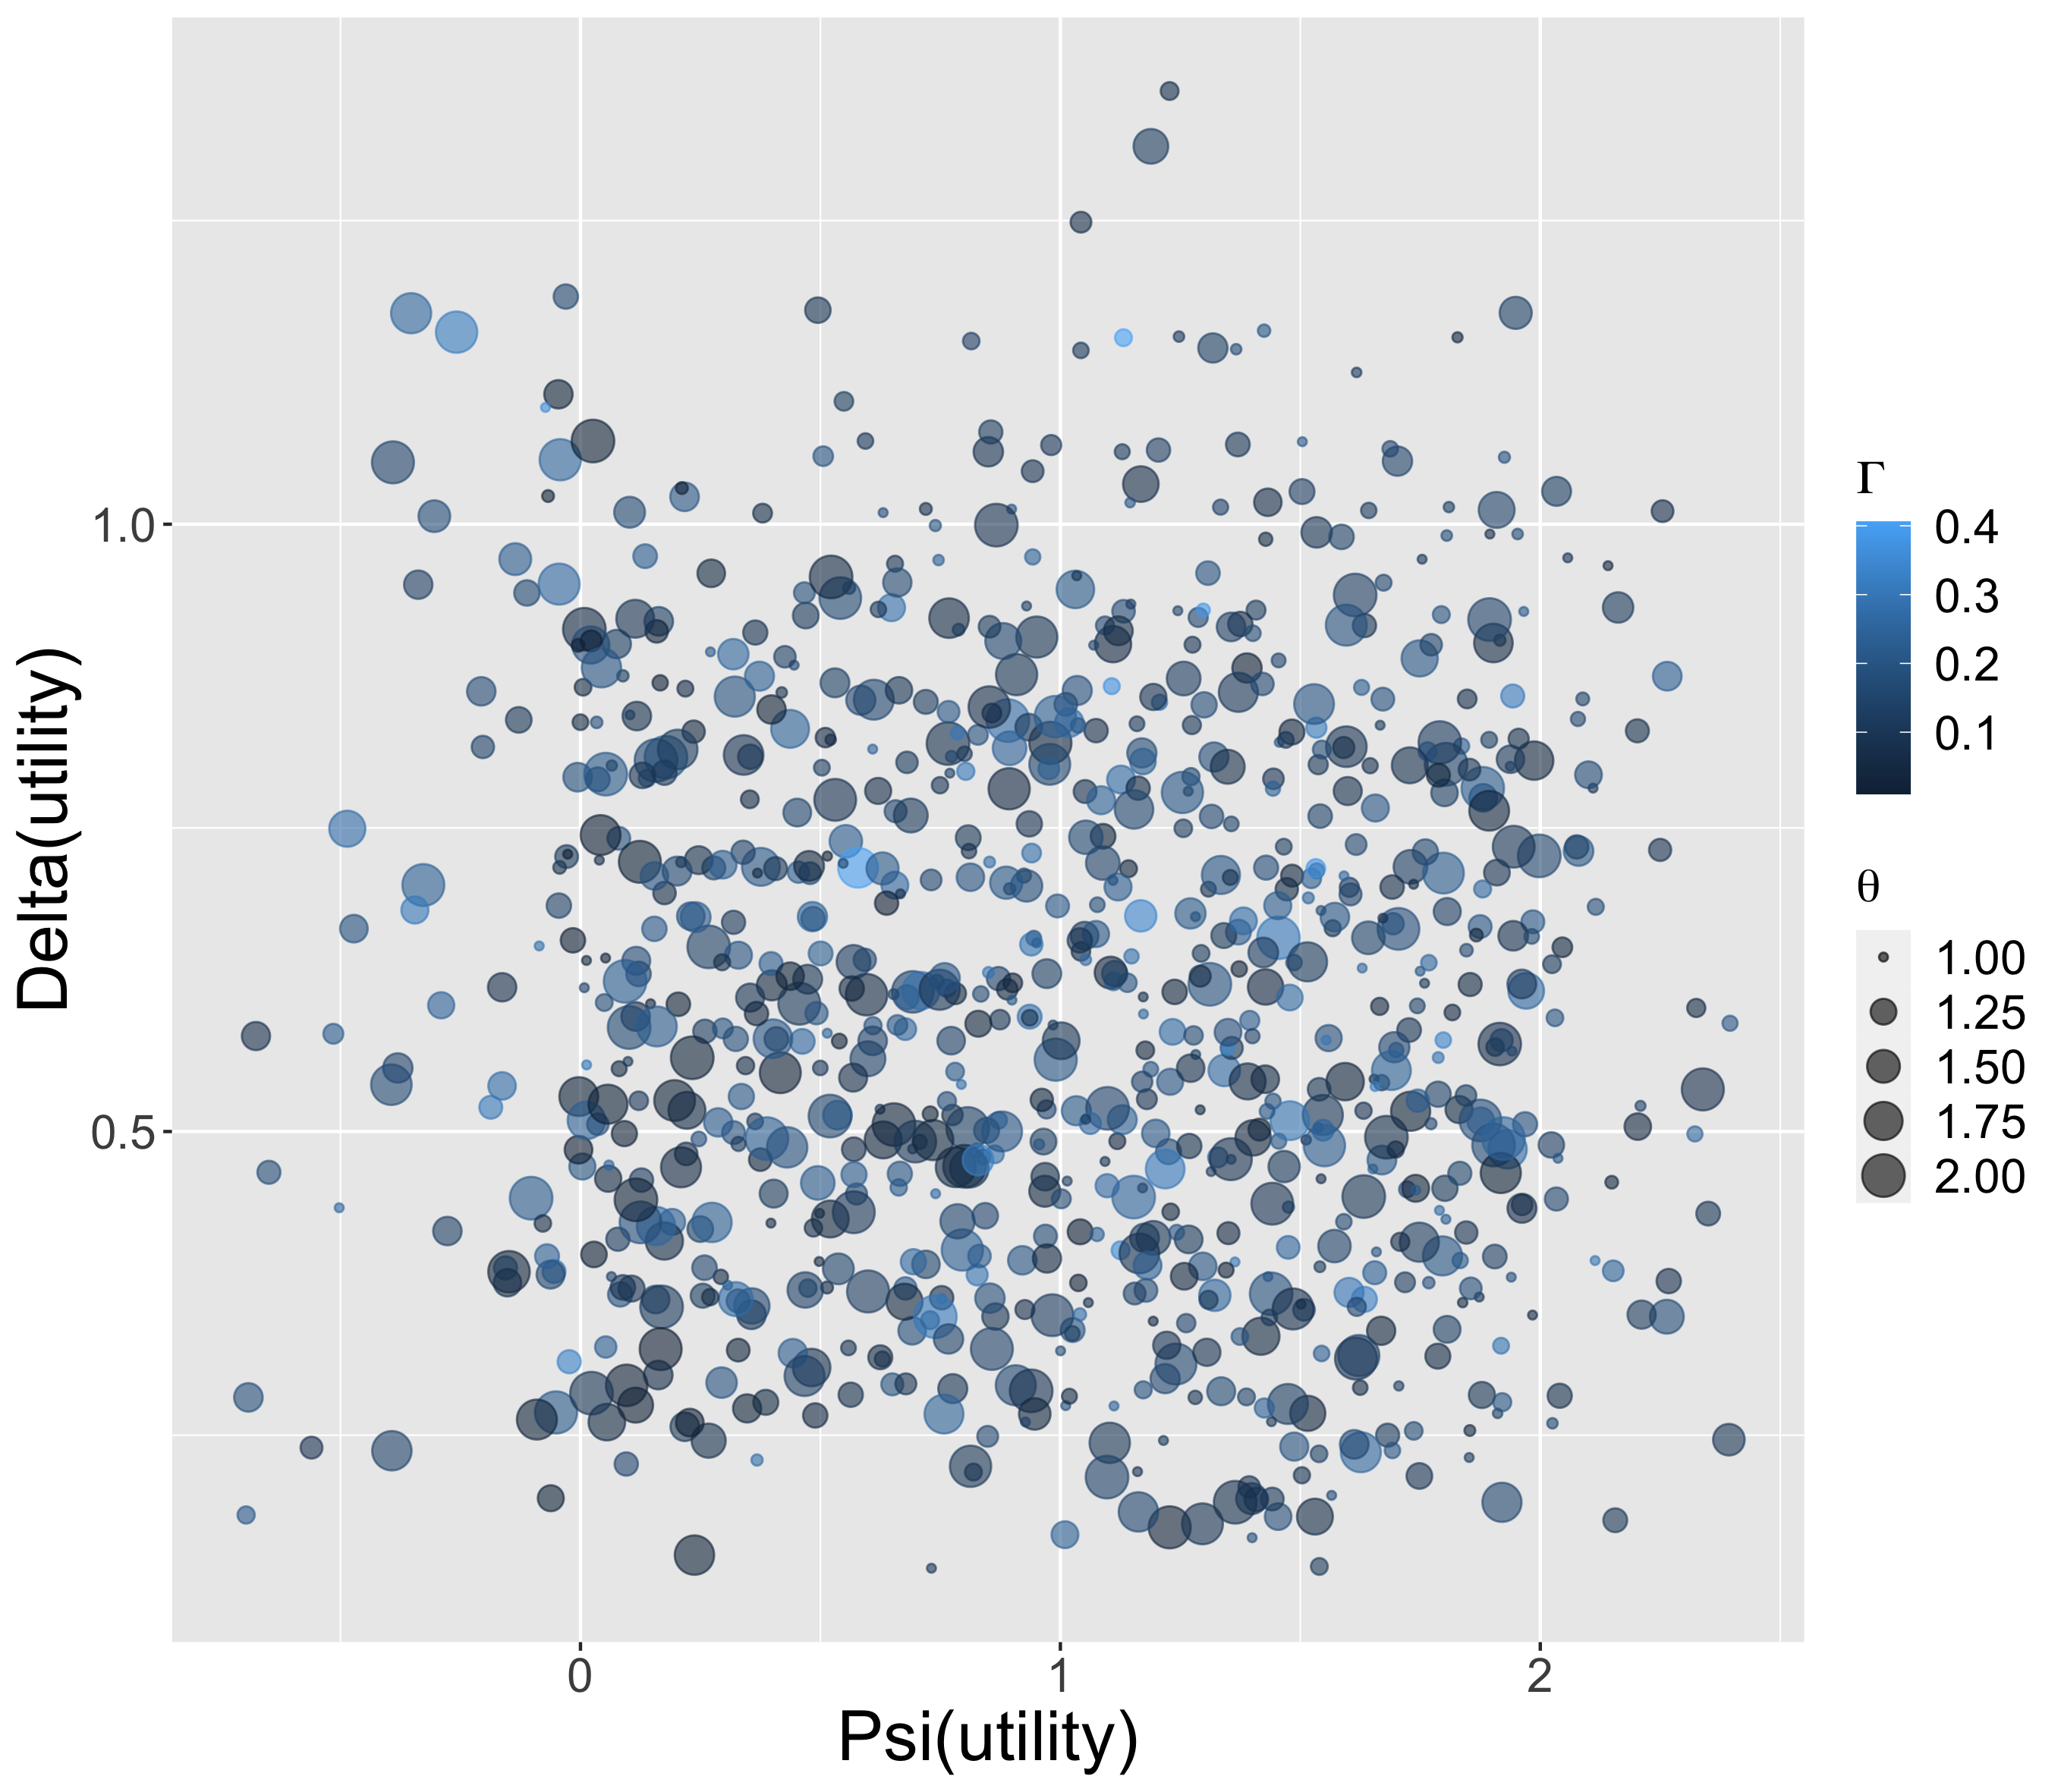
\includegraphics[width=0.49\textwidth]{../../../Papers/InnovationMultiscale/InnovationMultiscale-paper/figures/pse-psi-delta-utility_colorGamma_sizetheta.png}
\end{center}

\bigskip

(Left) bi-optimisation between contradictory objectives across scales; (Right) diversity of emergence regimes obtained with a diversity search algorithm


}


\sframe{Common aspects from simulation results}{

% First simulation results show that strong emergence appears in a significant number of regimes for the innovation model, and that contradictory objectives across scales can be simultaneously optimised using multi-objective genetic algorithms for both models.

$\rightarrow$ strong emergence quantified in a high diversity of regimes for the innovation diffusion model, probable (given cross-scale parameter influence, but not quantified) for the urban morphogenesis model

\bigskip

$\rightarrow$ optimisation objectives across scales seem generally contradictory, and can be simultaneously optimised with Pareto trade-offs

}




\sframe{Teaching 1: ontologies and feedbacks}{


% A few pitfalls have been identified while theoretically constructing the models and empirically exploring their parameter space using advanced model validation techniques with the OpenMOLE software (Reuillon et al., 2013): (i) to obtain a strong coupling between scales, and thus effective multiscalar dynamics rather than fixed effects at the meso scale only for example, both top-down and bottom-up feedbacks have to be included explicitly, and corresponding ontologies and processes must be identified; 

$\rightarrow$ models coupling scales with a single direction of inter-scale feedback can be simplified to non-stationary dynamics or fixed effects at a single scale: ``strong'' coupling is necessary

\bigskip

$\rightarrow$ scales have their own distinct ontologies with their own processes

\bigskip

% Q: is aggregation a process? not necessarily - but a feedback between variables

$\rightarrow$ inter-scales processes may be necessary to capture feedbacks and may necessitate their own ontology


}


\sframe{Teaching 2: consistent data parametrisation}{

%ii) the parametrisation or calibration with empirical data is significantly more cumbersome than with single level models, and synthetic systems are a first alternative to explore model behaviour; 

$\rightarrow$ model parametrisation with real data is more complicated: which scales? need of consistent datasets in case of multiple scales (cf Geodivercity project); how to consistently setup model states? \ldots

\bigskip

$\rightarrow$ synthetic systems of cities are a first way to explore model dynamics independently of geographical contingencies \cite{raimbault2019space}

}


\sframe{Teaching 3: stochasticity}{

% (iii) the convergence of model indicators regarding stochasticity seems more difficult to obtain, possibly due to non-linear noise propagation between scales; 

% histogram/distib for illustrated indicators for the innovation model? no time

\begin{center}
	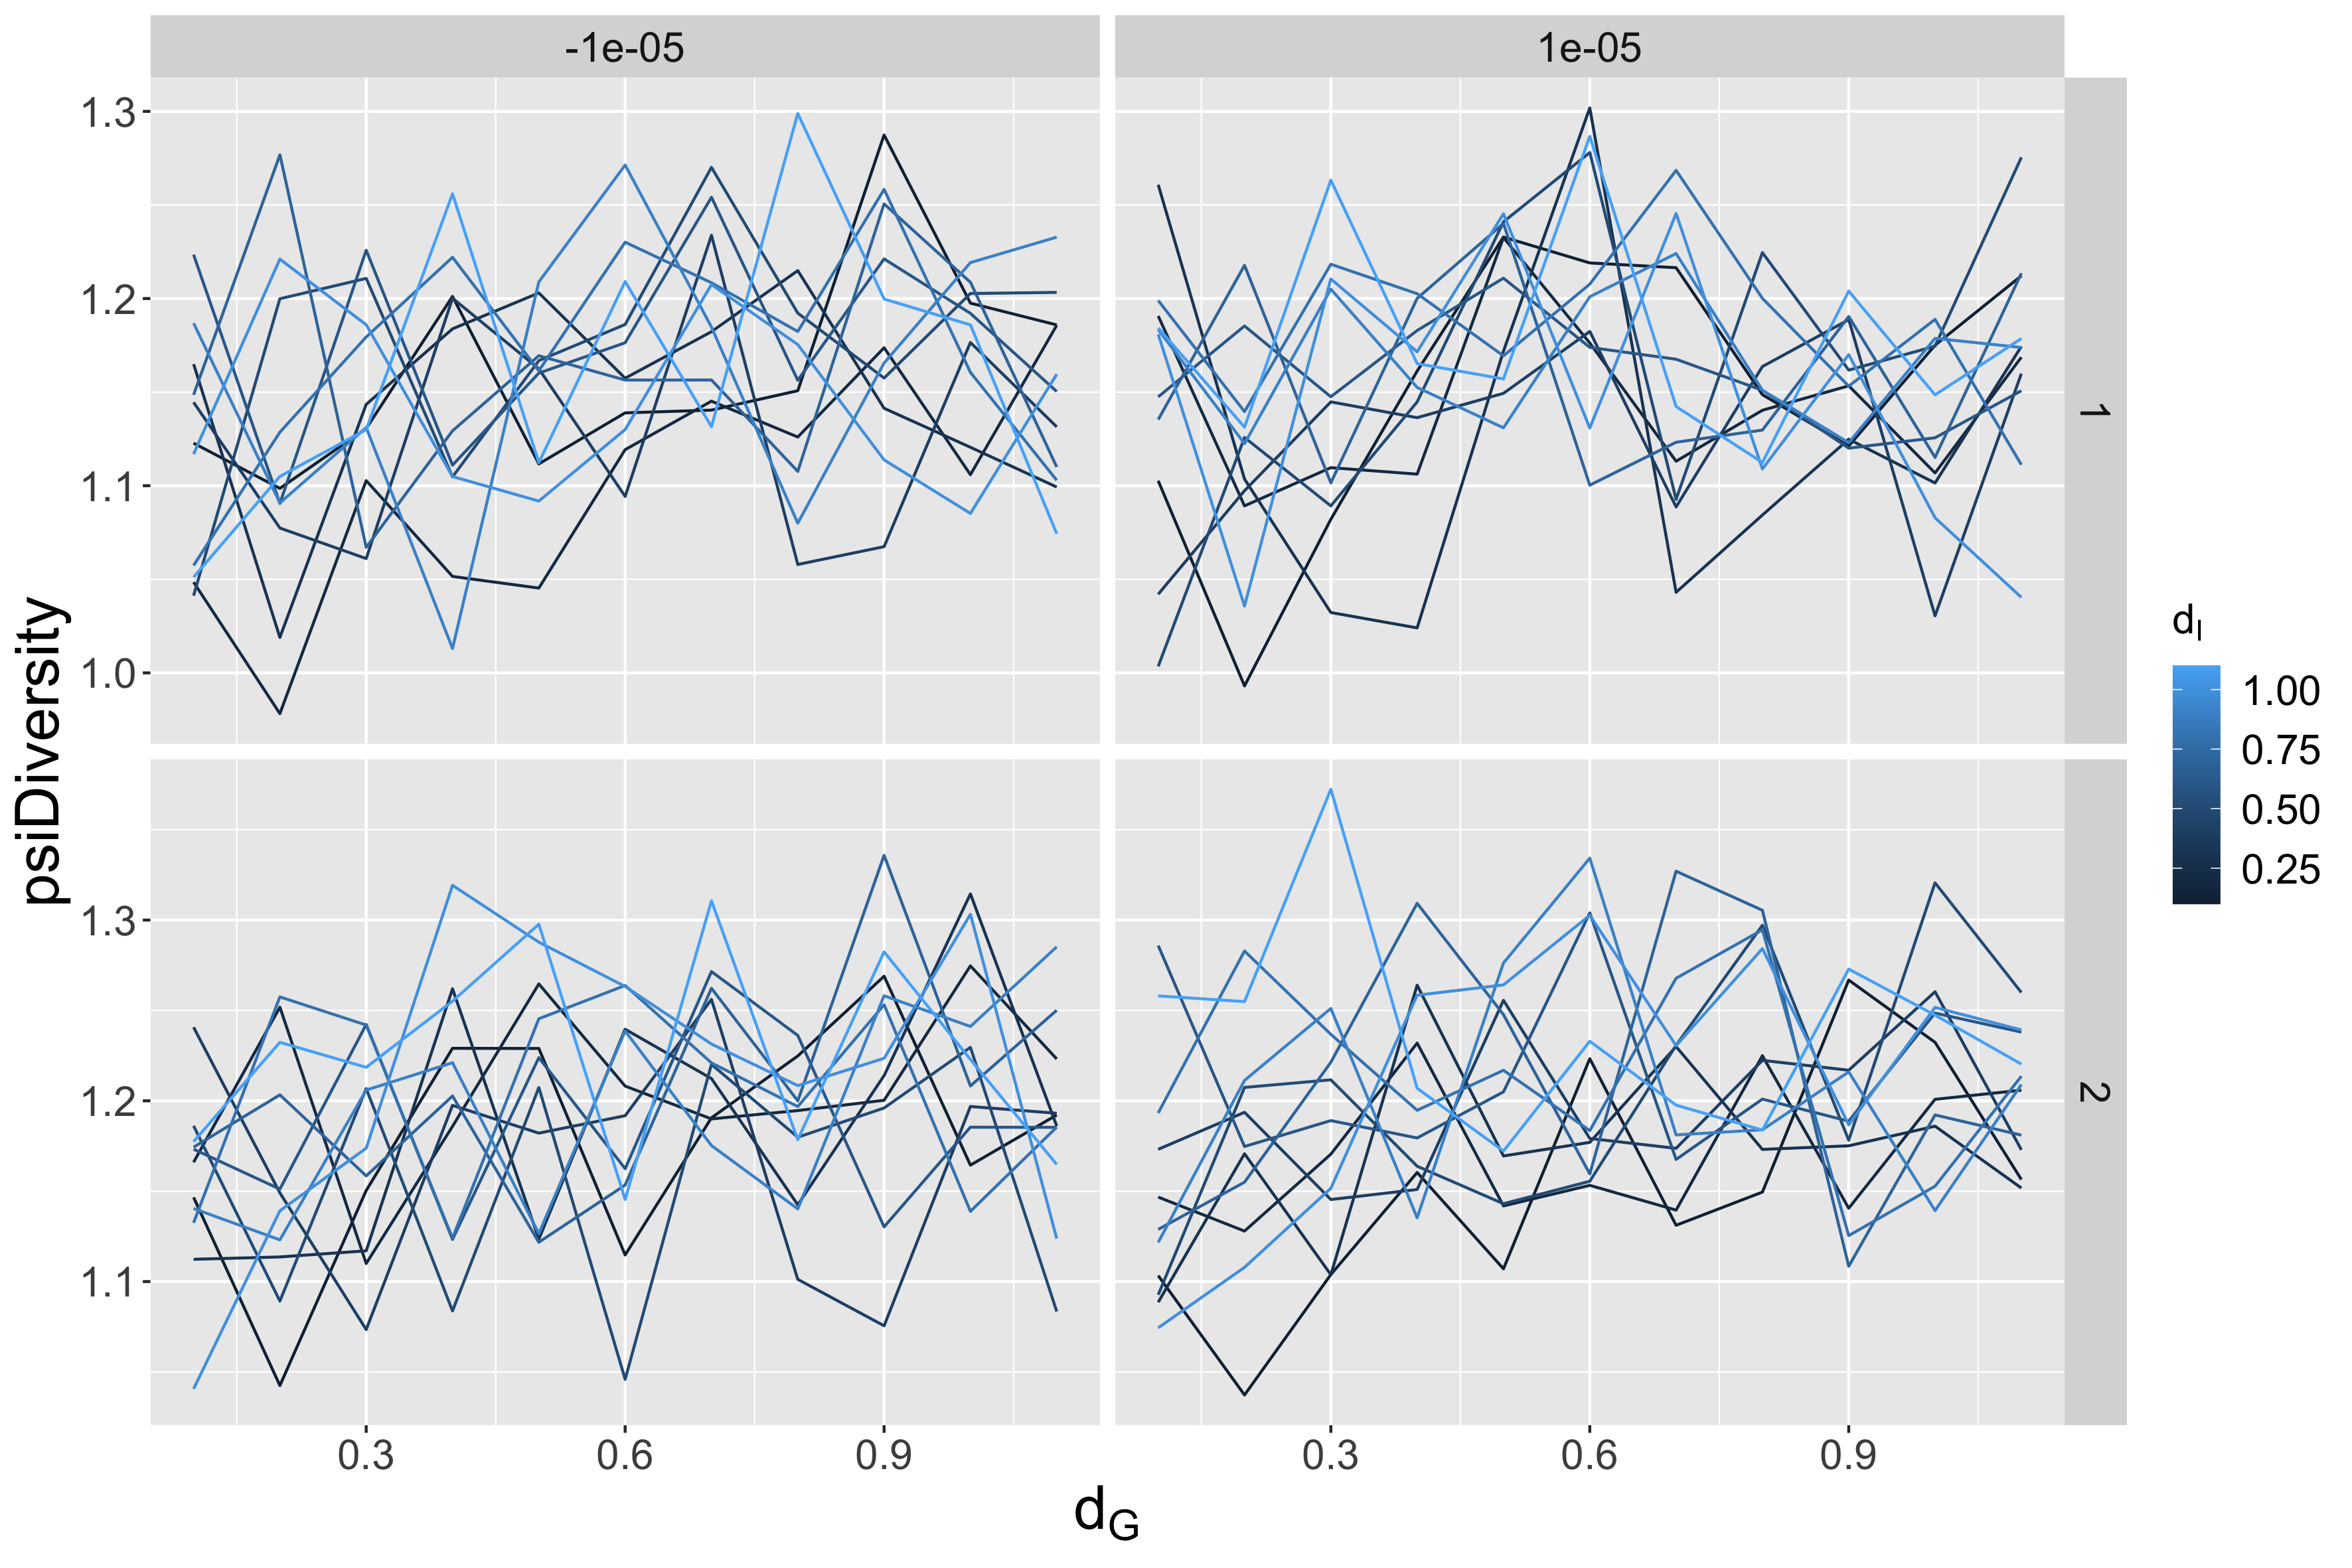
\includegraphics[width=0.49\textwidth]{../../../../Results/InnovationMultiscale/exploration/20230623_135234_EXPLORATION/psiDiversity_MED-macroGravityDecay_color-macroInnovationDecay_facet-mesoToMacroInnovationThreshold-macroToMesoExchangeMaxUpdate_mesoCrossOverProba05.png}
	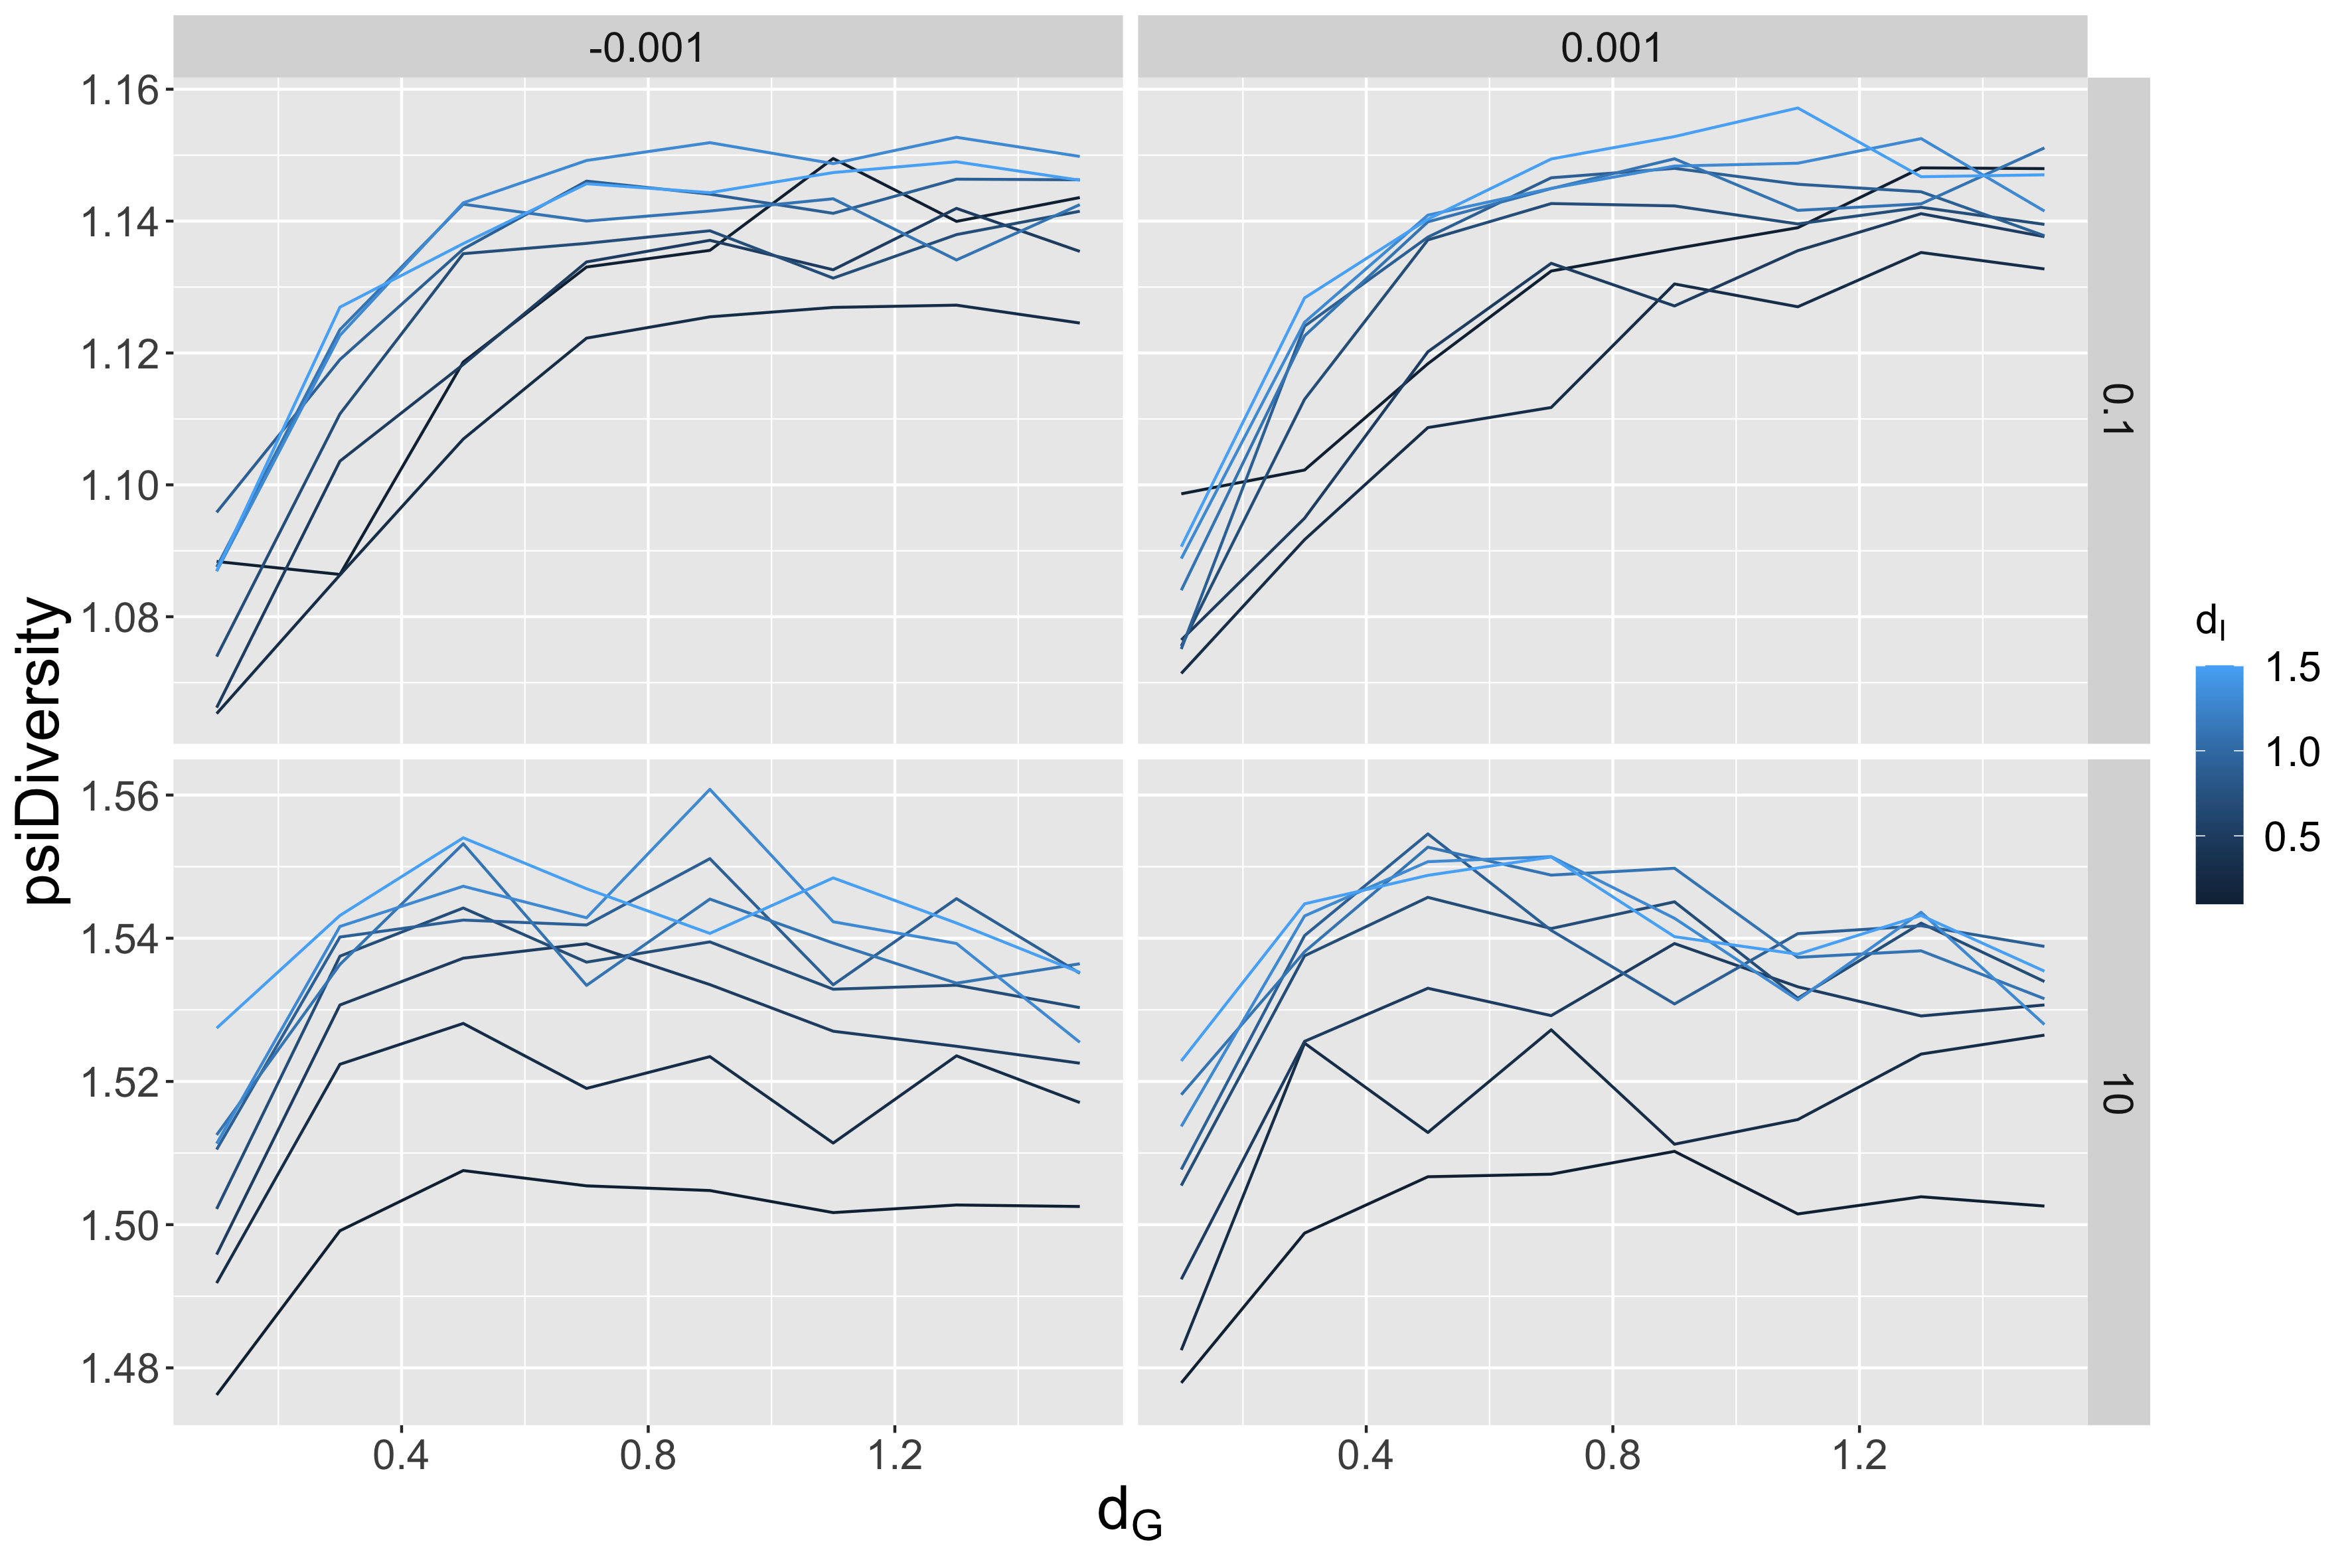
\includegraphics[width=0.49\textwidth]{../../../../Results/InnovationMultiscale/exploration/20230705-20230712_EXPLORATION/psiDiversity-macroGravityDecay_color-macroInnovationDecay_facet-mesoToMacroInnovationThreshold-macroToMesoExchangeMaxUpdate_mesoCrossOverProba05.png}
\end{center}

% not sure 100? check oms commit! -> 56547b137cb2e8c807511e71efde1c06ba42ef6d : 20 repets only!

$\rightarrow$ statistical convergence of indicators is more difficult to reach (example above for innovation diffusion: 20 vs 10,000 replications, despite ``good-looking'' empirical Sharpe ratios suggesting a low number of repetitions)

\bigskip

$\rightarrow$ non-linearities, fat-tail distribution, noise propagation between scales? More uncertainty-based/Bayesian validation methods?


}


\sframe{Teaching 4: quantifying strong emergence}{

% (iv) a crucial aspect remains to quantify the strength of emergence, such that these approaches are not a superfluous complication of simpler dynamics at a single scale – the indicators introduced by (Rosas et al., 2020) are good candidates for such measures but remain to be tested systematically on geosimulation models.

$\rightarrow$ issue of over-complication/overfitting (generic issue for simulation models \cite{raimbault2020indirect}): is the multi-scale aspect necessary?

\bigskip

$\rightarrow$ the stronger the emergence, the more it is needed? \cite{bedau2002downward}: for nominal emergence, can be simplified/surrogated; for weak emergence, depends on the cases? (cf Schelling model); for strong emergence difficult to be avoided because of the autonomy?

\bigskip

$\rightarrow$ need indicators and methods to systematically quantify emergence in multi-scalar simulated dynamics: cf. information-theory-based indicators proposed by \cite{rosas2020reconciling}

\bigskip

$\rightarrow$ link between strength of emergence and strength of coupling, and other types of complexities (such as \cite{pumain2003approche}'s ``interdisciplinary'' complexity), seems to be an open question, related to the nature of complexities \cite{raimbault2020relating} and complex knowledge/knowledge of the complex

}





\sframe{Discussion: still a long way to go!}{


%\textbf{Main results:}


\justify

$\rightarrow$ there seem to be methodological regularities when building strongly coupled multi-scale models - to what extent do they depend on the type of system, methodological framework, do they hold with a parametrisation on real data?
			
\bigskip

$\rightarrow$ subtle compromise between model complication/complexity and the effective capture of multi-scale dynamics

\bigskip

$\rightarrow$ application to multi-scalar policies still far, but already possible in a stylised way such as for trade-offs between SDGs (at a single scale for now \cite{raimbault2022trade})

\bigskip
\bigskip

%\textbf{Conclusion: } 

\textbf{Open repositories for presented models:}

\texttt{https://github.com/JusteRaimbault/UrbanGrowth}

\texttt{https://github.com/JusteRaimbault/InnovationMultiscale-model}

}









%%%%%%%%%%%%%%%%%%%%%
\begin{frame}[allowframebreaks]
\frametitle{References}
\bibliographystyle{apalike}
\bibliography{biblio}
\end{frame}
%%%%%%%%%%%%%%%%%%%%%%%%%%%%




\end{document}









